\section{Proactive Caching for Spatial Queries in Mobile Environments}

\subsection{Introduction}

\begin{frame}
\frametitle{Introduction}
	\begin{center}
	\Large
	Published at: ICDE '05: Proceedings of the 21st International Conference on Data Engineering\\\vspace{1em}
	by\\\vspace{1em}
	Haibo Hu, Jianliang Xu, Wing Sing Wong, Baihua Zheng, Dik Lun Lee, and Wang-Chien Lee\\\vspace{1em}
	April 2005
	\end{center}
\end{frame}


\begin{frame}
\frametitle{Motivation}
\large


\end{frame}


\begin{frame}
\frametitle{Related Work}
\Large

Caching:
\begin{itemize}\itemsep 16pt
\item Page Caching
\item Semantic Caching
\end{itemize}

\end{frame}

%----------------------------------------------


\subsection{Problem}

\begin{frame}
\frametitle{Problem}

\end{frame}

\begin{frame}
\frametitle{R-Tree}

\begin{center}
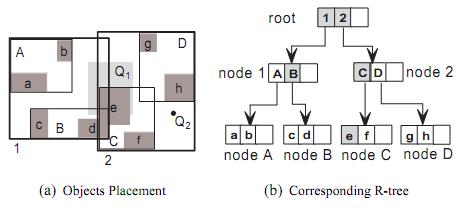
\includegraphics[scale=0.95]{images/r-tree.jpg}
\end{center}
\end{frame}

%----------------------------------------------

\subsection{Contribution}

\begin{frame}
\frametitle{Proactive Caching}

\begin{enumerate}
\item Execute query $Q$ on local partial R-tree index and cache
\item If any items are found while executing $Q$ locally, then return immidiately
\item If $Q$ is satisfied then terminate, else Construct $Q_r = Q + H$ and send to server
\end{enumerate}

\begin{center}
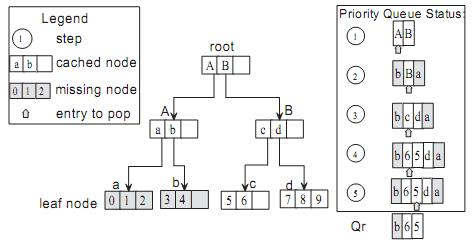
\includegraphics[scale=0.55]{images/kNNproactive-caching.jpg}
\end{center}

\end{frame}

\begin{frame}
\frametitle{Proactive Caching}

\begin{center}
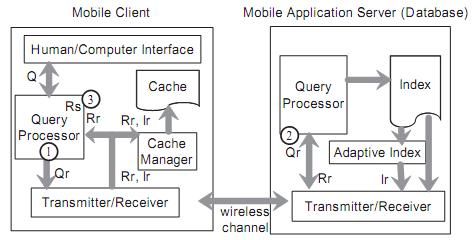
\includegraphics[scale=0.80]{images/proactive-caching.jpg}
\end{center}

\end{frame}

\begin{frame}
\frametitle{Response time and Hit rate}

Query responsetime:\\
$resp(Q)=\frac{|R_r|(T{Q_{r}}+\frac{1}{2}|R_r|\cdot T_d}{|R|}$
\vspace{1.5em}

Cache Hit rate:\\
$hit_c = \frac{|R_s|}{R}$
\end{frame}


\begin{frame}
\frametitle{}

Algorithm is a 2-approximation algorithm

When cached node is removed, the children of that item should be considered into the benifit calculations.

$\sum_{j \in D(i)}{prob(j)\times size(i)+ prob(i)\times size(i)}$


\end{frame}


%----------------------------------------------

\subsection{Experimental Results}
%
%\begin{frame}
%\frametitle{Setting}
%\end{frame}
%
%\begin{frame}
%
%\end{frame}
%
%\begin{frame}
%\frametitle{Cache hit ratio / Data Size - scope 1 and 2}
%
%\end{frame}
%
%\begin{frame}
%\frametitle{Cache hit ratio / Query interval - scope 1 and 2}
%
%\end{frame}
%
%\begin{frame}
%\frametitle{Cache hit ratio / Moving interval - scope 1 and 2}
%%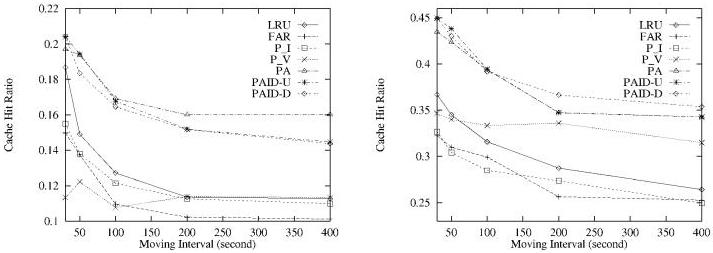
\includegraphics[scale=0.5]{images/fig9.jpg}
%
%\end{frame}
%

\begin{frame}
\frametitle{Conclusion}
\Large
Proactive Caching outperforms page caching and semantic caching
\end{frame}

\begin{frame}
\frametitle{Impression}

Their results were not stellar\\

Graphs are "`cut"' just before compeditors might seem to become better

\end{frame}